As detailed in Section \ref{sec:th}, Moltres compiles with the MOOSE Navier-Stokes
\cite{peterson_overview_2018} and Heat Transfer modules for incompressible flow
modeling capabilities by default. Moltres couples with these modules natively because they are all
built on the MOOSE framework.

% Past work with Moltres have modeled incompressible salt flow and temperature advection-diffusion
% with the \gls{INS} or \gls{INSAD} implementations of
% the Navier-Stokes equations. Coupling with compressible, porous media, and
% finite volume implementations within the Navier-Stokes module is possible through native
% \gls{MOOSE} multiphysics coupling capabilities but has not been demonstrated yet.

To address the lack of turbulence modeling in Moltres, I implemented a \gls{SA} turbulence model
\cite{spalart_one-equation_1994}, described in Section \ref{sec:lit-turb}, with \gls{SUPG}
stabilization on Moltres. On balance the \gls{SA} model is a complete (does not require prior
knowledge of the actual turbulence behavior) and computationally efficient one-equation turbulence
model for approximating wall-bounded turbulent flows. The \gls{SA} model implementation in Moltres
couples seamlessly with the continuous \gls{FEM} \gls{INSAD} \cite{lindsay_automatic_2021} model
from the Navier-Stokes module. Alongside the \gls{SA} model, Moltres also now has turbulent
diffusion physics kernels for temperature and the delayed neutron precursors.

The SA model in Moltres follows the \gls{SA} model with rotation correction (SA-R) implementation
\cite{aupoix_extensions_2003, dacles-mariani_numericalexperimental_1995} as described on the
\gls{NASA} Turbulence Modeling Resource website \cite{rumsey_turbulence_nodate}. The $f_{t2}$
term is togglable using the \texttt{use\_ft2\_term} input parameter (false by default). Moltres'
implementation solves for the modified dynamic viscosity $\tilde{\mu}$ as follows:

\begin{gather}
  \rho \frac{\partial\tilde{\mu}}{\partial t} + \rho \mathbf{u}\cdot\nabla\tilde{\mu} = \rho c_{b1}
  \left(1-f_{t2}\right)\tilde{S}\tilde{\mu} + \frac{1}{\sigma}\{\nabla\cdot\left[\left(\mu+
  \tilde{\mu}\right)\nabla\tilde{\mu}\right] + c_{b2}|\nabla\tilde{\mu}|^2\} - \left(c_{w1}f_w -
  \frac{c_{b1}}{\kappa^2}f_{t2}\right)\left(
  \frac{\tilde{\mu}}{d}\right)^2
  \shortintertext{where}
  \begin{align*}
    \mu_t &= \tilde{\mu}f_{v1} = \text{turbulent eddy viscosity}, &
    f_{v1} &= \frac{\chi^3}{\chi^3 + c_{v1}^3}, \\
    \chi &= \frac{\tilde{\mu}}{\mu}, &
    \tilde{S} &= \Omega + \frac{\tilde{\nu}}{\kappa^2 d^2} f_{v2}, \\
    f_{v2} &= 1 - \frac{\chi}{1+\chi f_{v1}}, &
    \Omega &= \sqrt{2W_{ij}W_{ij}} = \text{vorticity magnitude}, \\
    W_{ij} &= \frac{1}{2}\left(\frac{\partial u_i}{\partial x_j} - \frac{\partial u_j}{\partial x_i}
    \right), &
      f_w &= g\left(\frac{1 + c_{w3}^6}{g^6 + c_{w3}^6}\right)^{1/6}, \\
      g &= r + c_{w2}\left(r^6 - r\right), &
      r &= \text{min}\left(\frac{\tilde{\nu}}{\tilde{S}\kappa^2d^2}, 10\right), \\
      f_{t2} &= c_{t3} \exp{\left(-c_{t4}\chi^2\right)},
  \end{align*}
\shortintertext{and the constants are}
  \sigma = \frac{2}{3}, \ c_{b1} = 0.1355, \ c_{b2} = 0.622, \ \kappa = 0.41, \
  c_{w1} = \frac{c_{b1}}{\kappa^2} + \frac{1+c_{b2}}{\sigma}, \nonumber \\
  c_{w2} = 0.3, \ c_{w3} = 2, \
  c_{v1} = 7.1, \ c_{t3} = 1.2, \ c_{t4} = 0.5 \ \text{.} \nonumber
\end{gather}

The \gls{SA} model is verified simple verification and validation tests of the \gls{SA} model in Moltres using
reference problems for channel, pipe, and \gls{BFS} flow. The Moltres test dataset is available on
Zenodo \cite{park_dataset_2023}. The following subsections show plots comparing
results from Moltres to reference data from literature.

\subsection{Turbulent Channel Flow Verification Test}

The channel flow test is based on the \gls{DNS} of turbulent channel flow
with Re$_\tau\approx395$ by Moser et al.\ \cite{moser_direct_1999}. Corresponds to Re = 13750.

\begin{figure}[htb!]
  \centering
  \begin{subfigure}[b]{0.48\columnwidth}
    \centering
    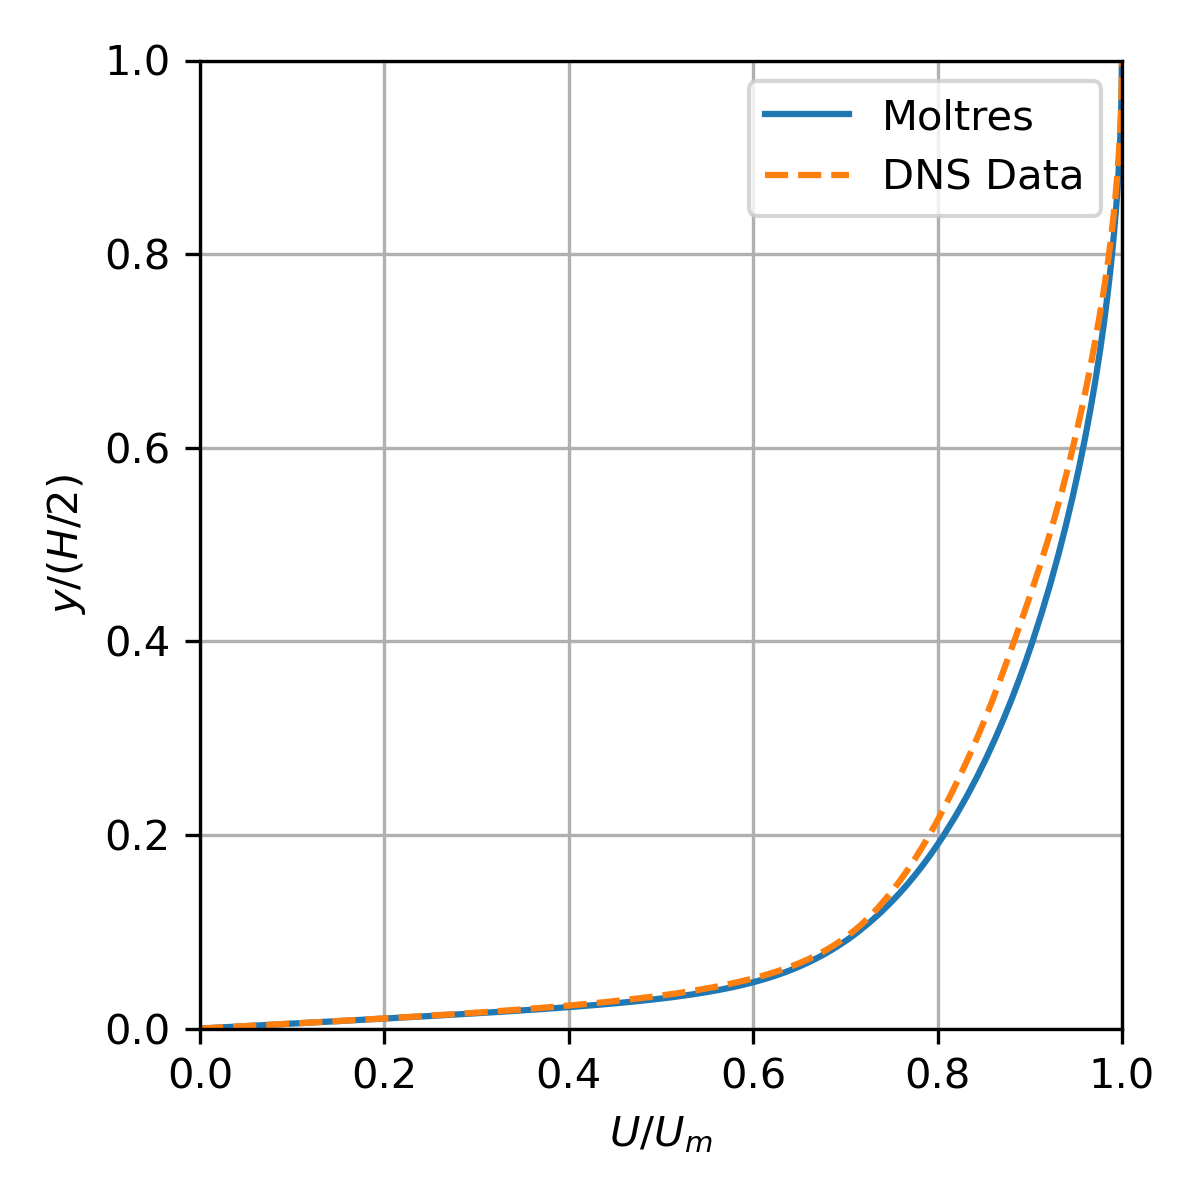
\includegraphics[width=\columnwidth]{channel_vel}
    \caption{Normalized velocity distribution across the channel.}
    \label{fig:}
  \end{subfigure}
  \hfill
  \begin{subfigure}[b]{0.48\columnwidth}
    \centering
    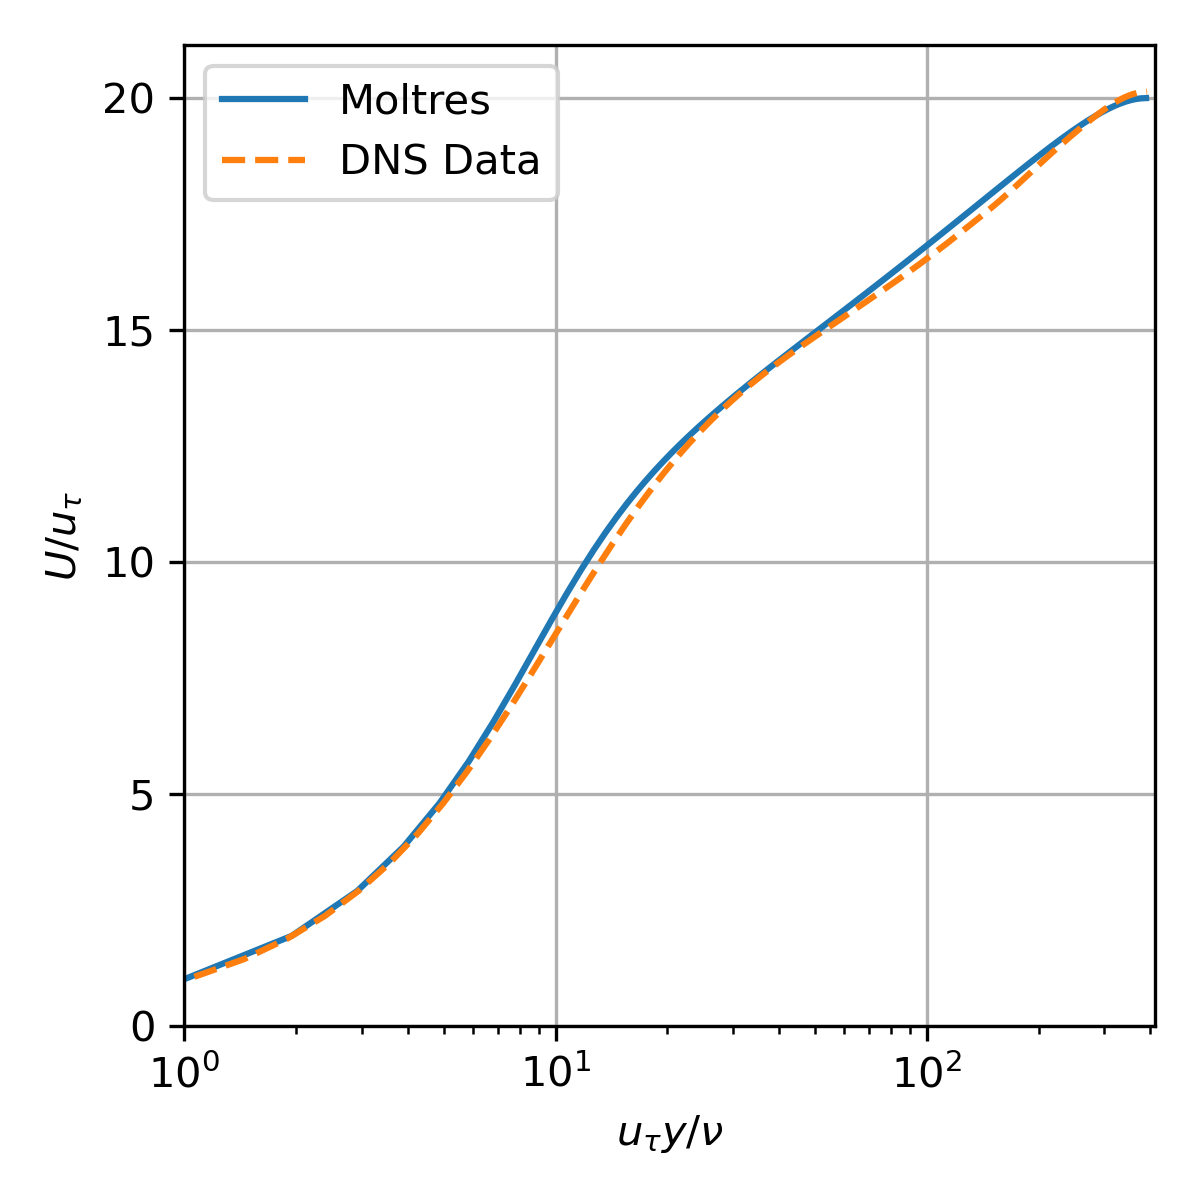
\includegraphics[width=\columnwidth]{channel_nondim}
    \caption{Dimensionless velocity vs.\ dimensionless wall distance.}
    \label{fig:}
  \end{subfigure}
  \begin{subfigure}[b]{0.48\columnwidth}
    \centering
    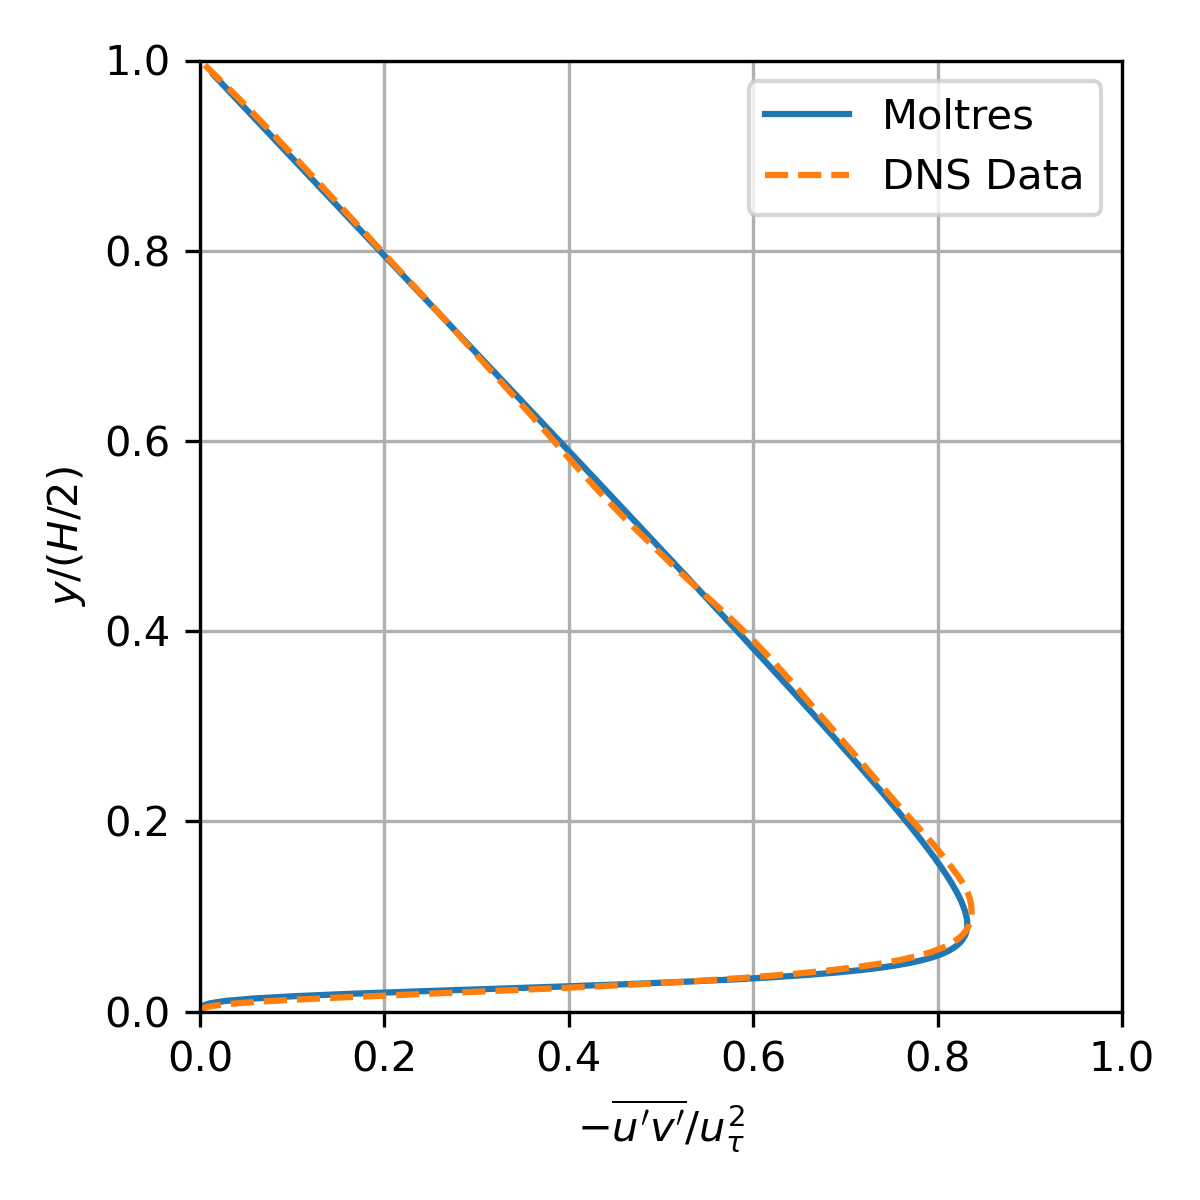
\includegraphics[width=\columnwidth]{channel_stress}
    \caption{Normalized stress distribution across the channel.}
    \label{fig:}
  \end{subfigure}
  \caption{Comparison of turbulent channel flow results at Re$_\tau\approx395$ against reference
  \gls{DNS} results \cite{moser_direct_1999}.}
  \label{fig:}
\end{figure}

\subsection{Turbulent Pipe Flow Validation Test}

The pipe flow test is based on the turbulent pipe flow experiment with Re $\approx 40000$ by
Laufer \cite{laufer_structure_1954}.

\begin{figure}[htb]
  \centering
  \begin{subfigure}[b]{0.48\columnwidth}
    \centering
    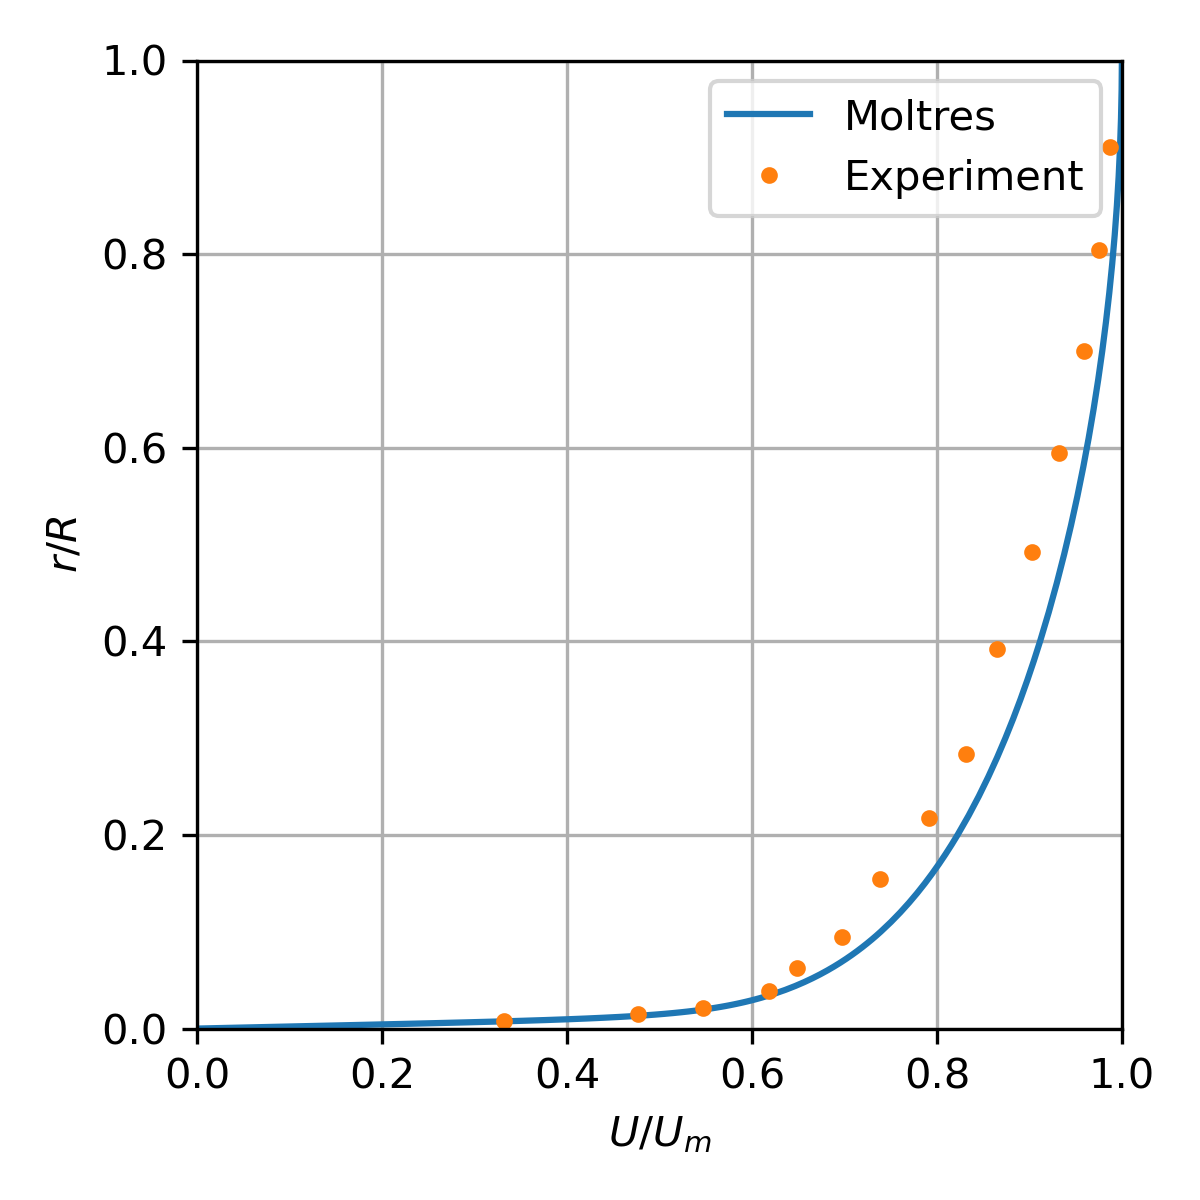
\includegraphics[width=\columnwidth]{pipe_vel}
    \caption{Normalized velocity distribution across the pipe.}
    \label{fig:}
  \end{subfigure}
  \hfill
  \begin{subfigure}[b]{0.48\columnwidth}
    \centering
    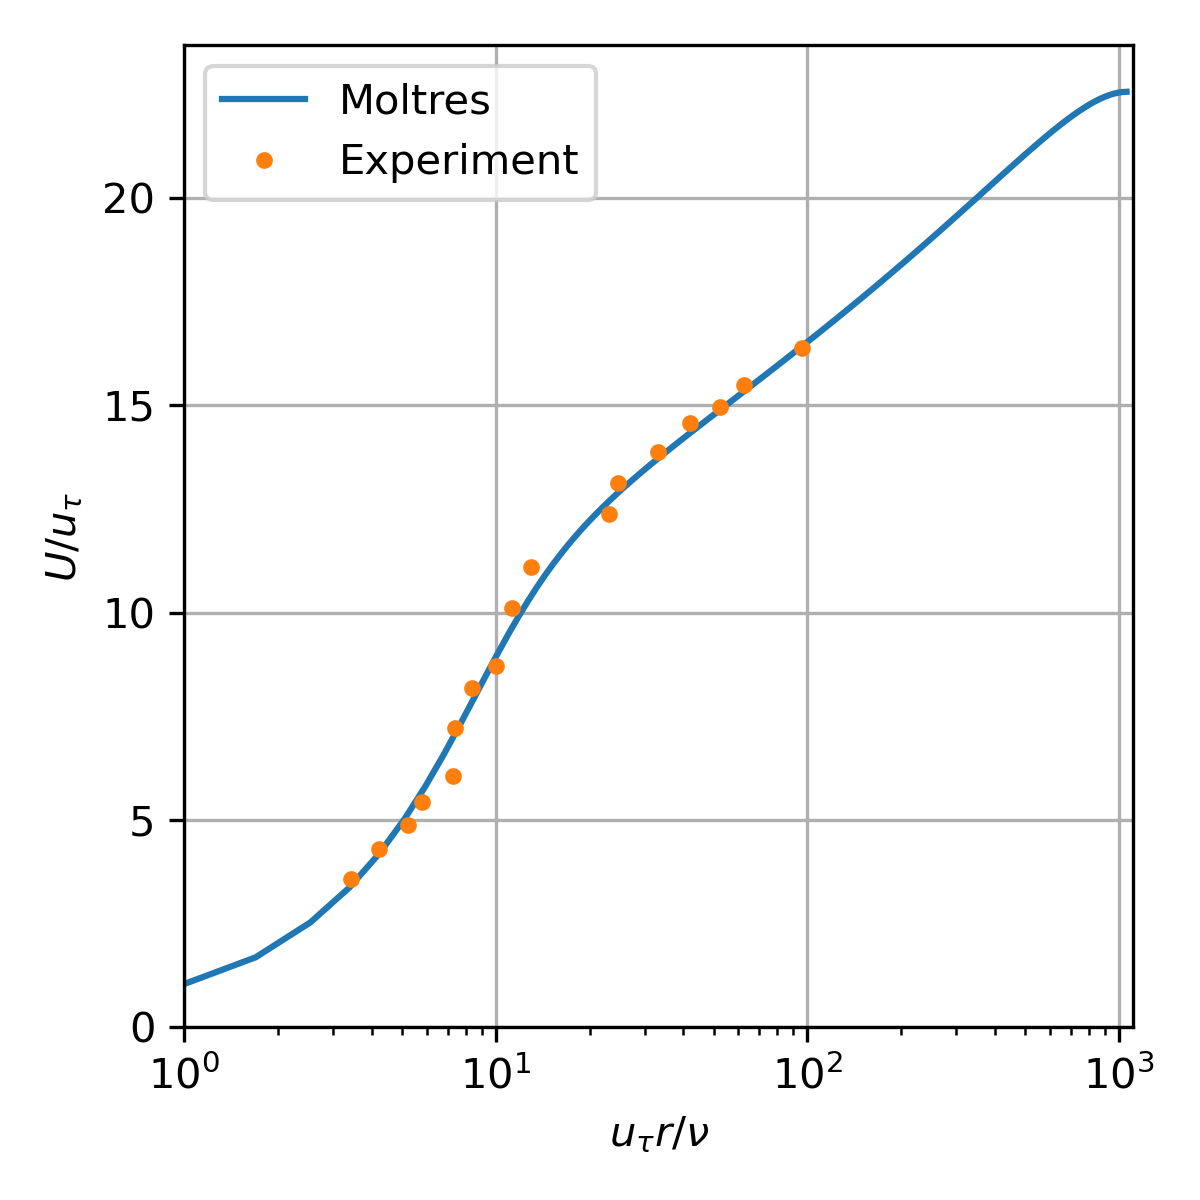
\includegraphics[width=\columnwidth]{pipe_nondim}
    \caption{Dimensionless velocity vs.\ dimensionless wall distance}
    \label{fig:}
  \end{subfigure}
  \begin{subfigure}[b]{0.48\columnwidth}
    \centering
    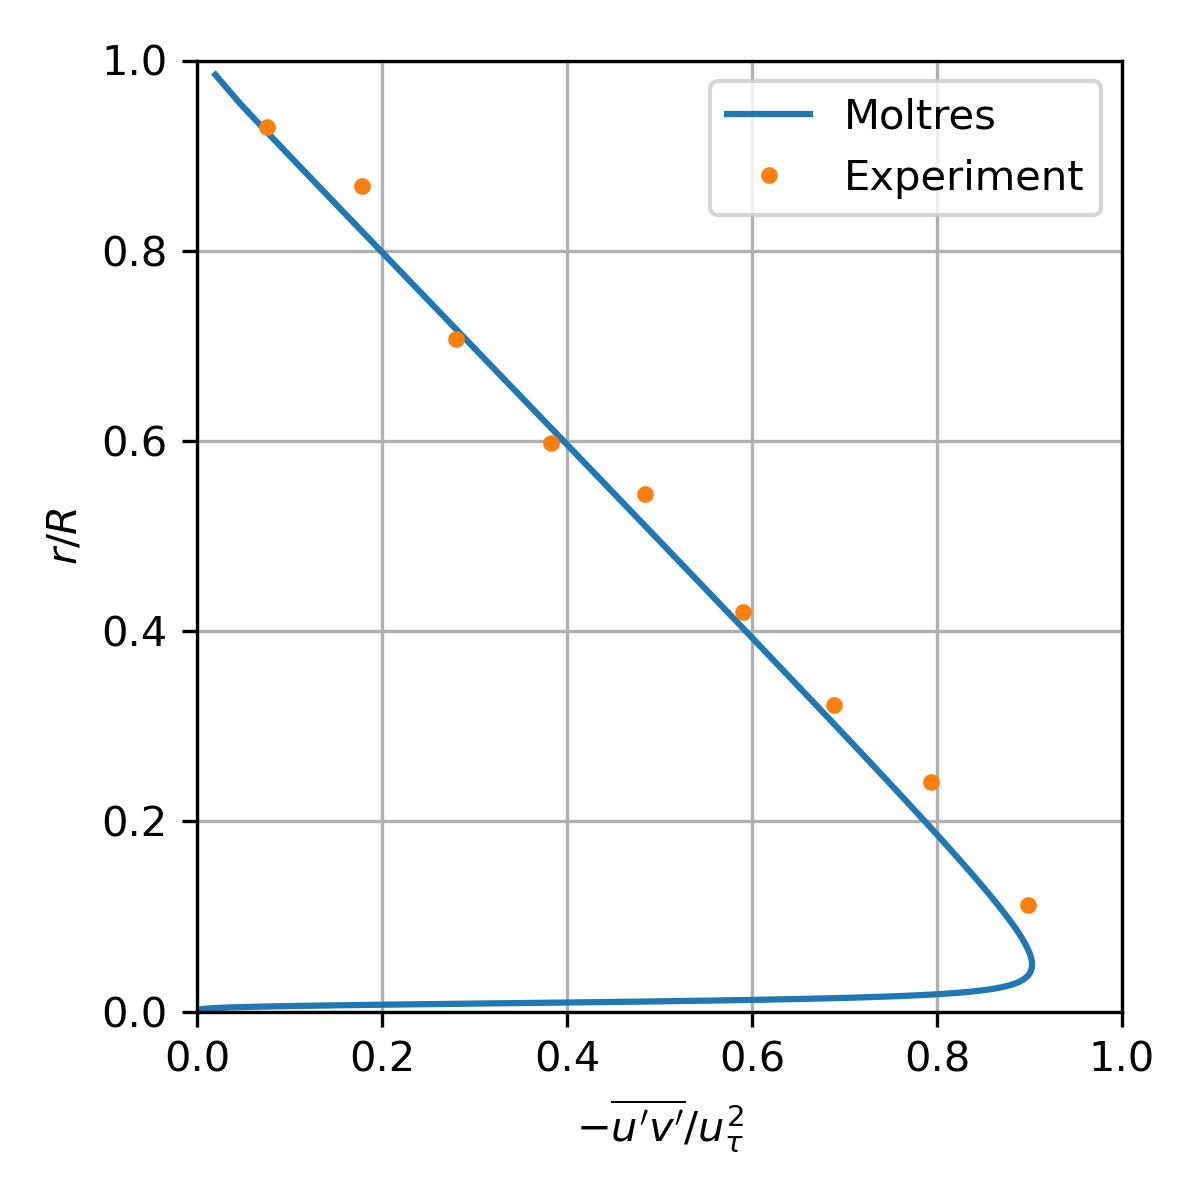
\includegraphics[width=\columnwidth]{pipe_stress}
    \caption{Normalized turbulent shear stress distribution across the pipe.}
    \label{fig:}
  \end{subfigure}
  \caption{Comparison of turbulent pipe flow results at Re $\approx 40000$ against reference
  experimental data \cite{laufer_structure_1954}.}
\end{figure}

\subsection{Backward-Facing Step Flow Validation Test}

The \gls{BFS} flow test is based on the BFS flow experiment with Re $\approx36000$ by Driver \&
Seegmiller \cite{driver_features_1985}. The \gls{SA} model implementation in Moltres performs
largely similarly to the reference SA model results
provided on the \gls{NASA} Turbulence Modeling Resource website \cite{rumsey_turbulence_nodate}.

\begin{table}[htb]
  \centering
  \small
  \caption{\gls{BFS} flow reattachment length estimates normalized by step height $H$.}
  \begin{tabular}{l c c c}
    \toprule
    & {Experimental data \cite{driver_features_1985}} & {Reference \gls{SA} model
  \cite{rumsey_turbulence_nodate}} & {Moltres \gls{SA} model} \\
    \midrule
    Reattachment length [-] & {$6.26 \pm 0.10$} & 6.1 & 6.36 \\
    \bottomrule
  \end{tabular}
  \label{table:bfs}
\end{table}

\begin{figure}[htb]
  \centering
  \hfill
  \begin{subfigure}[b]{0.4\columnwidth}
    \centering
    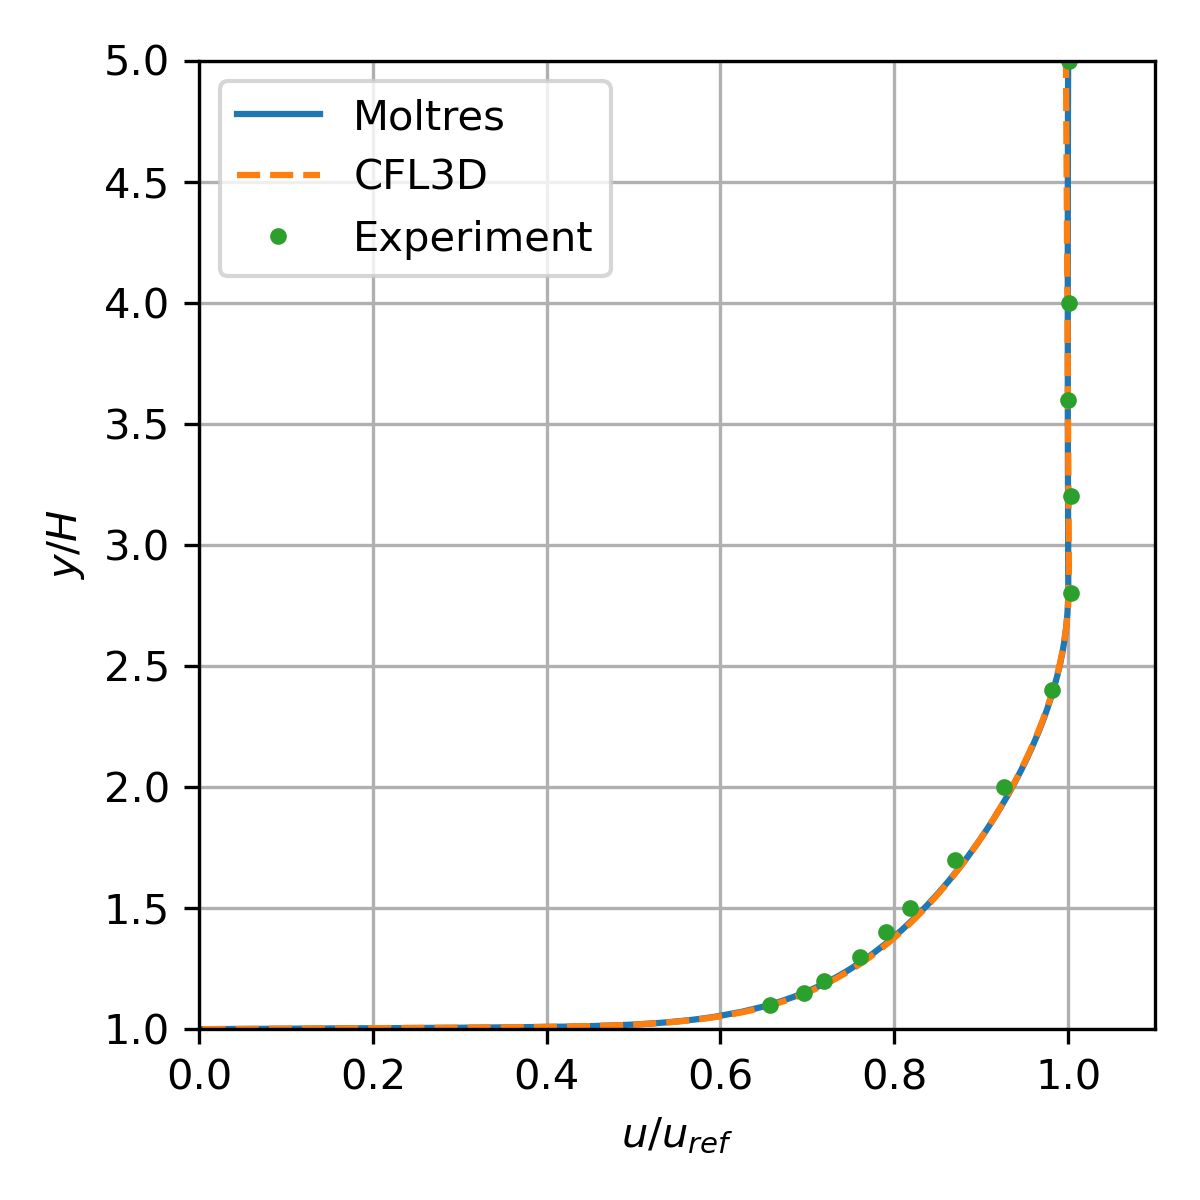
\includegraphics[width=\columnwidth]{bfs_upstream_vel}
    \caption{Normalized velocity distribution at $x/H=-4$ upstream of step.}
    \label{fig:}
  \end{subfigure}
  \hfill
  \begin{subfigure}[b]{0.4\columnwidth}
    \centering
    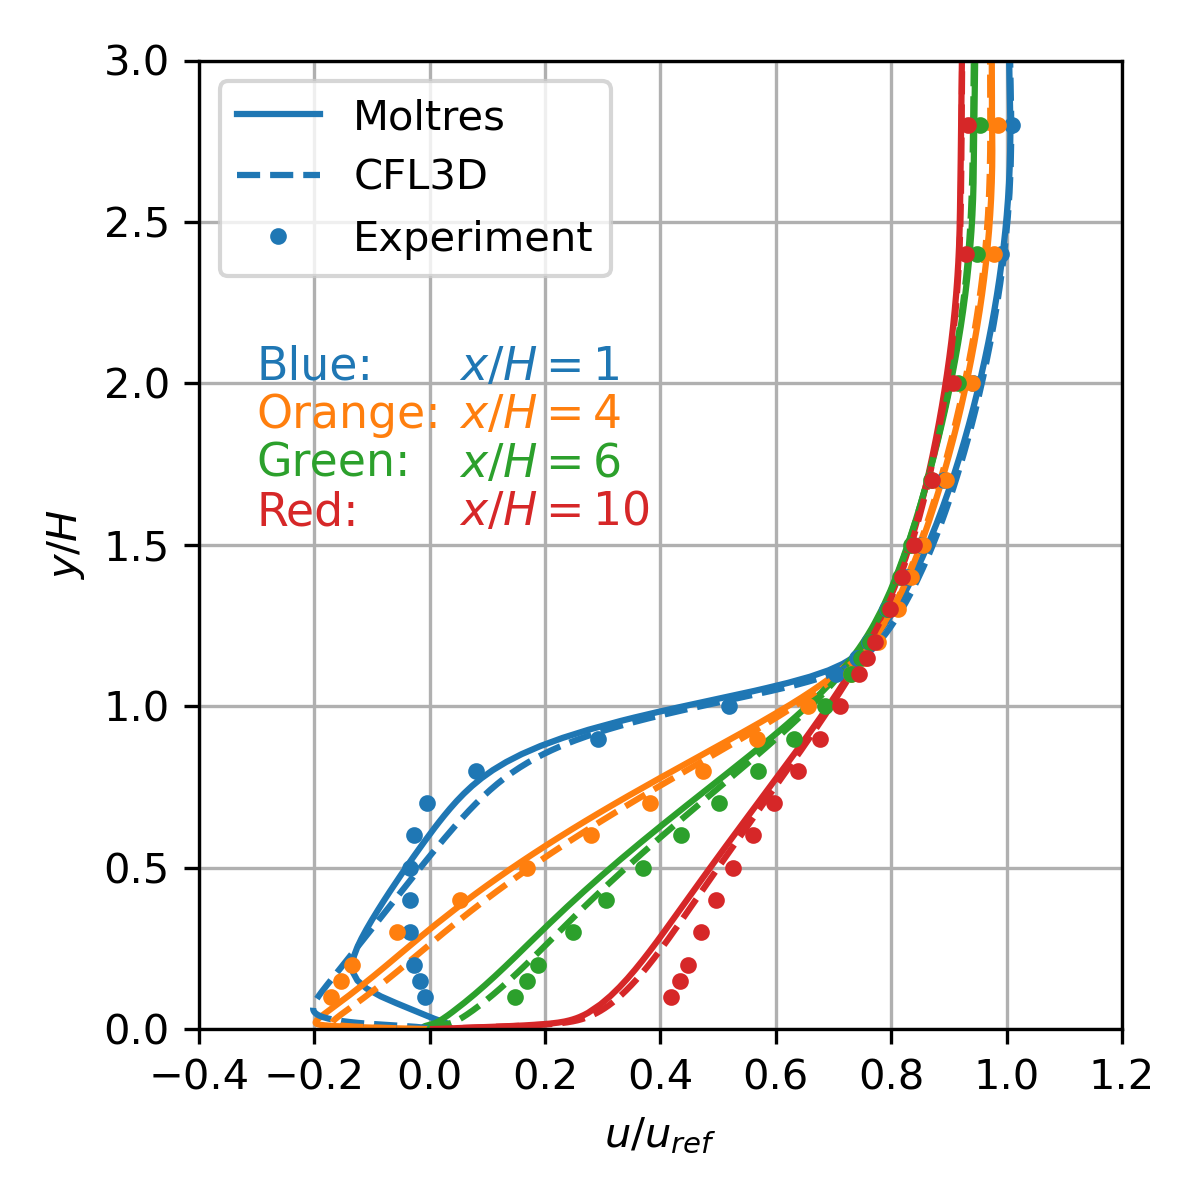
\includegraphics[width=\columnwidth]{bfs_downstream_vel}
    \caption{Normalized velocity distribution at various $x/H$ locations downstream of step.}
    \label{fig:}
  \end{subfigure} \hfill \\
  \centering
  \hfill
  \begin{subfigure}[b]{0.4\columnwidth}
    \centering
    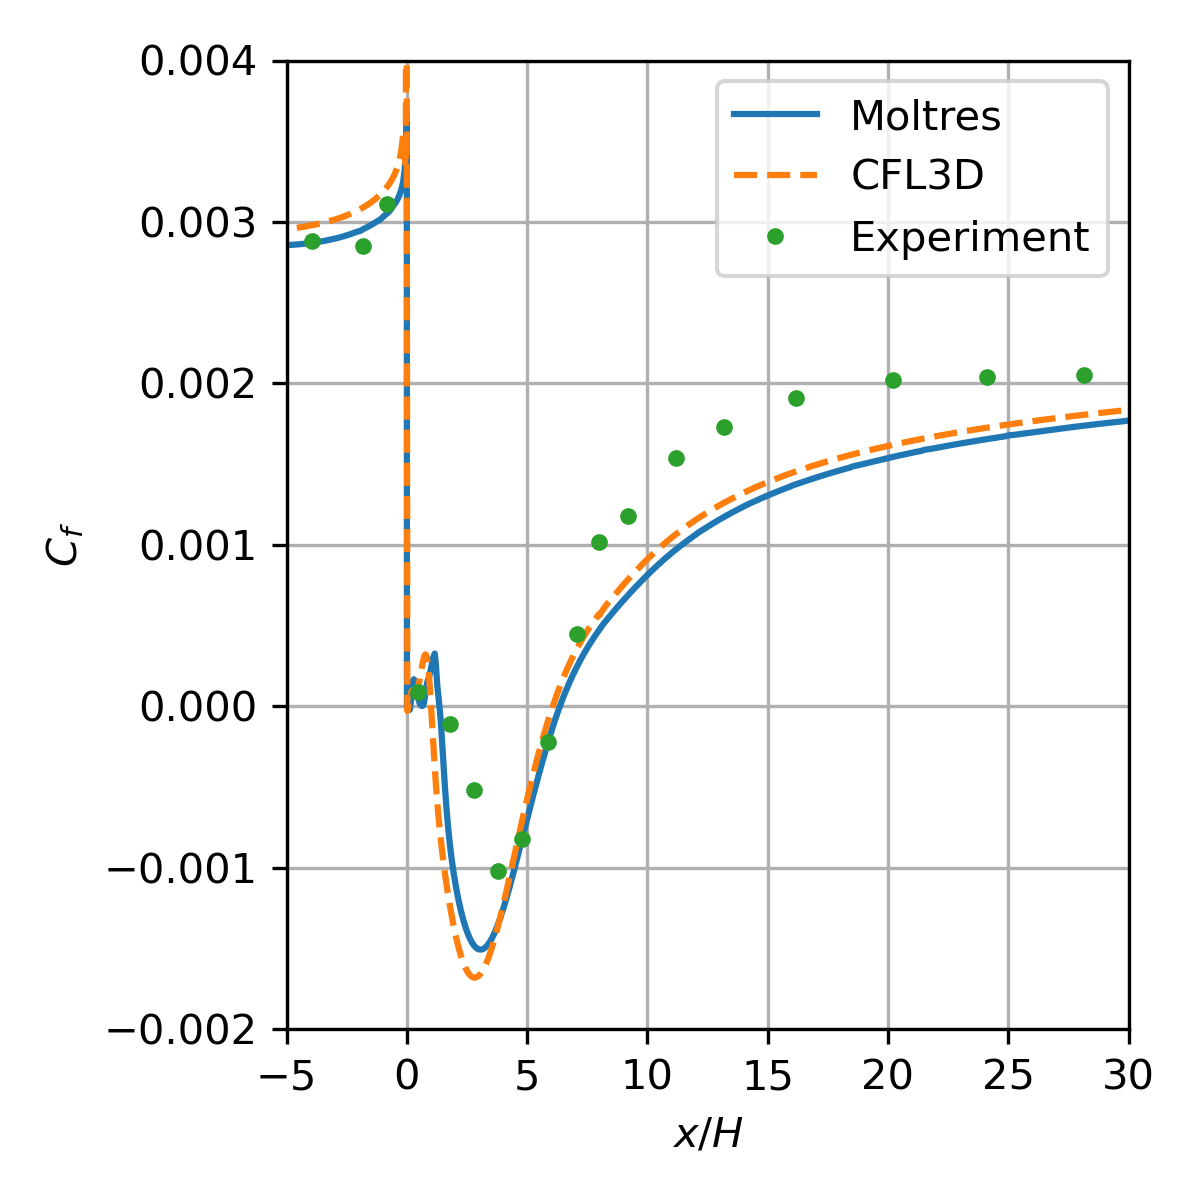
\includegraphics[width=\columnwidth]{bfs_cf}
    \caption{Skin friction coefficient along the bottom wall.}
    \label{fig:}
  \end{subfigure}
  \hfill
  \begin{subfigure}[b]{0.4\columnwidth}
    \centering
    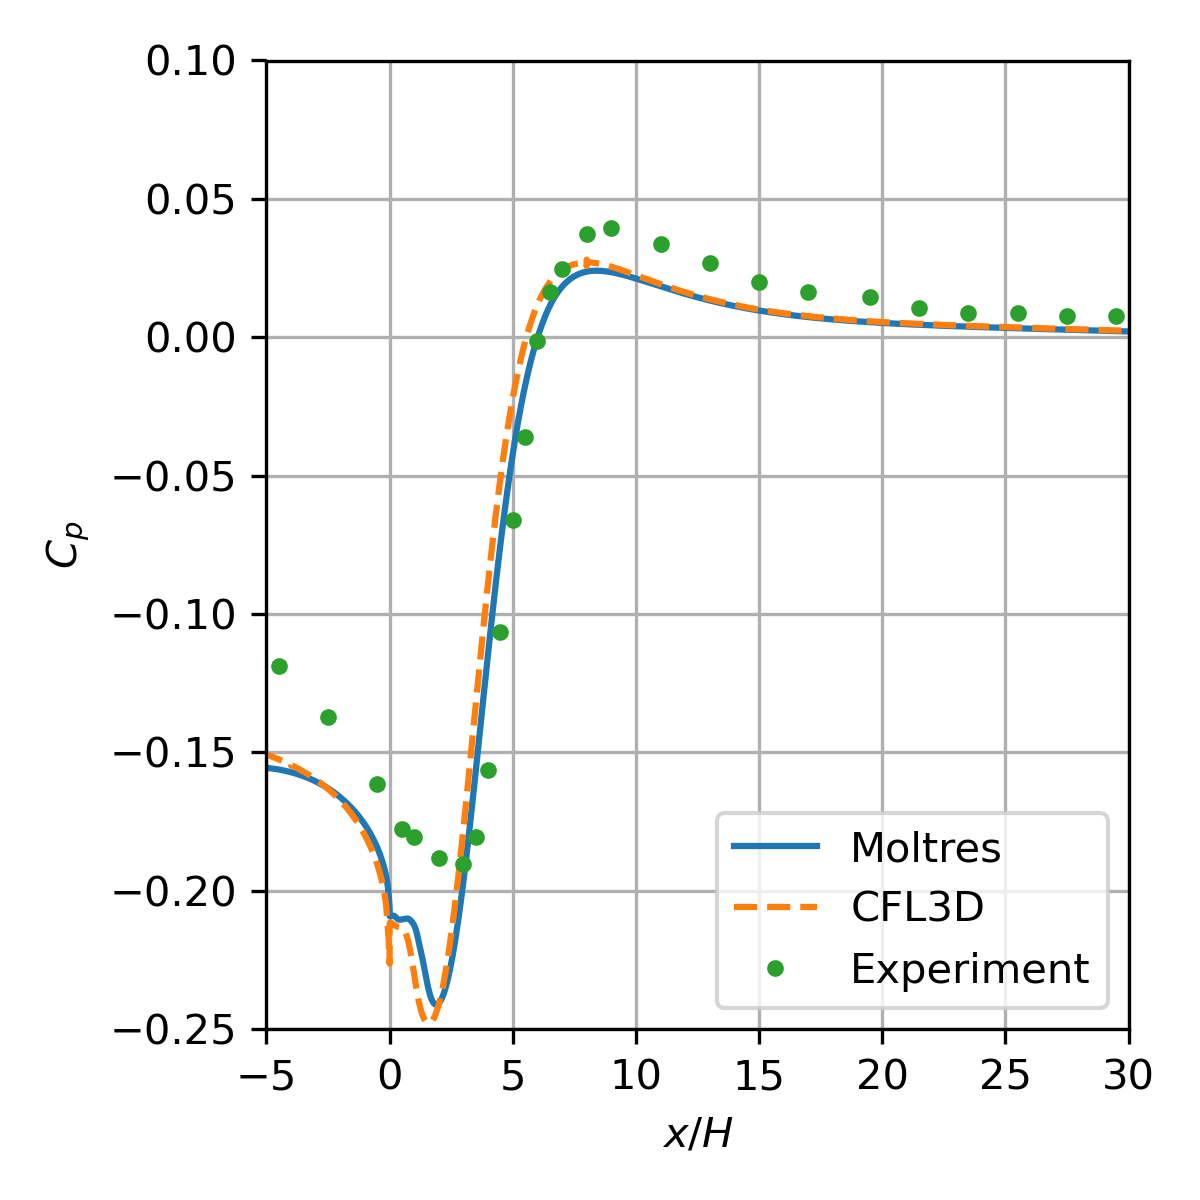
\includegraphics[width=\columnwidth]{bfs_cp}
    \caption{Skin pressure coefficient along the bottom wall.}
    \label{fig:}
  \end{subfigure} \hfill \\
  \centering
  \begin{subfigure}[b]{0.4\columnwidth}
    \centering
    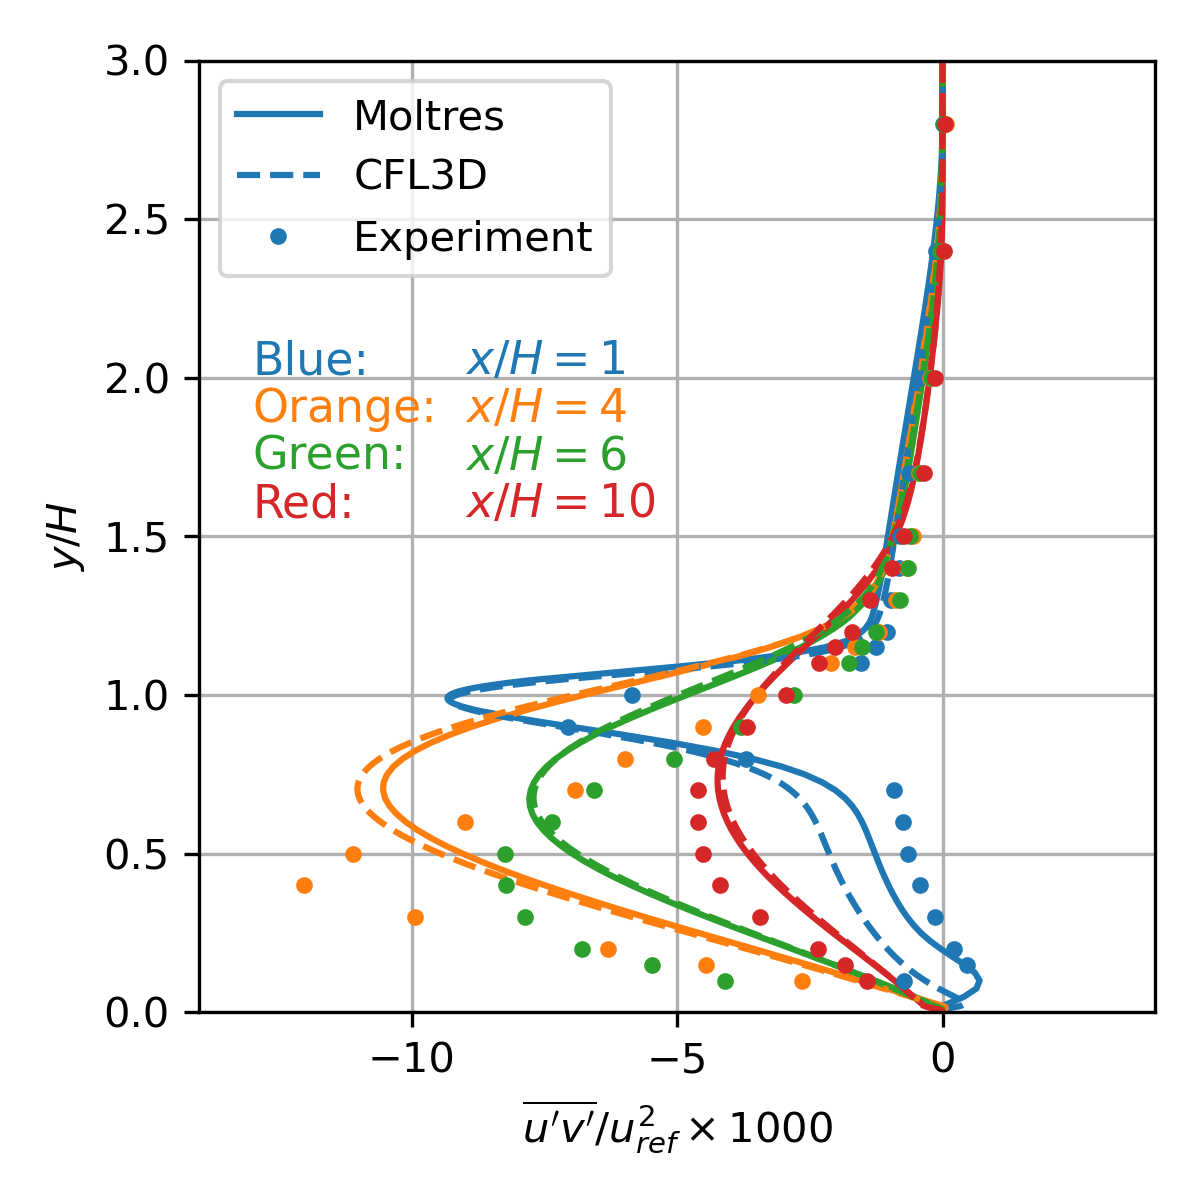
\includegraphics[width=\columnwidth]{bfs_stress}
    \caption{Normalized turbulent shear stress distribution at various $x/H$ locations downstream
    of step.}
    \label{fig:}
  \end{subfigure}
  \caption{Comparison of backward facing step flow results at Re $\approx 36000$ against reference
  experimental data and computational data from the CFL3D code.}
  \label{fig:}
\end{figure}

\begin{figure}[htb!]
  \centering
  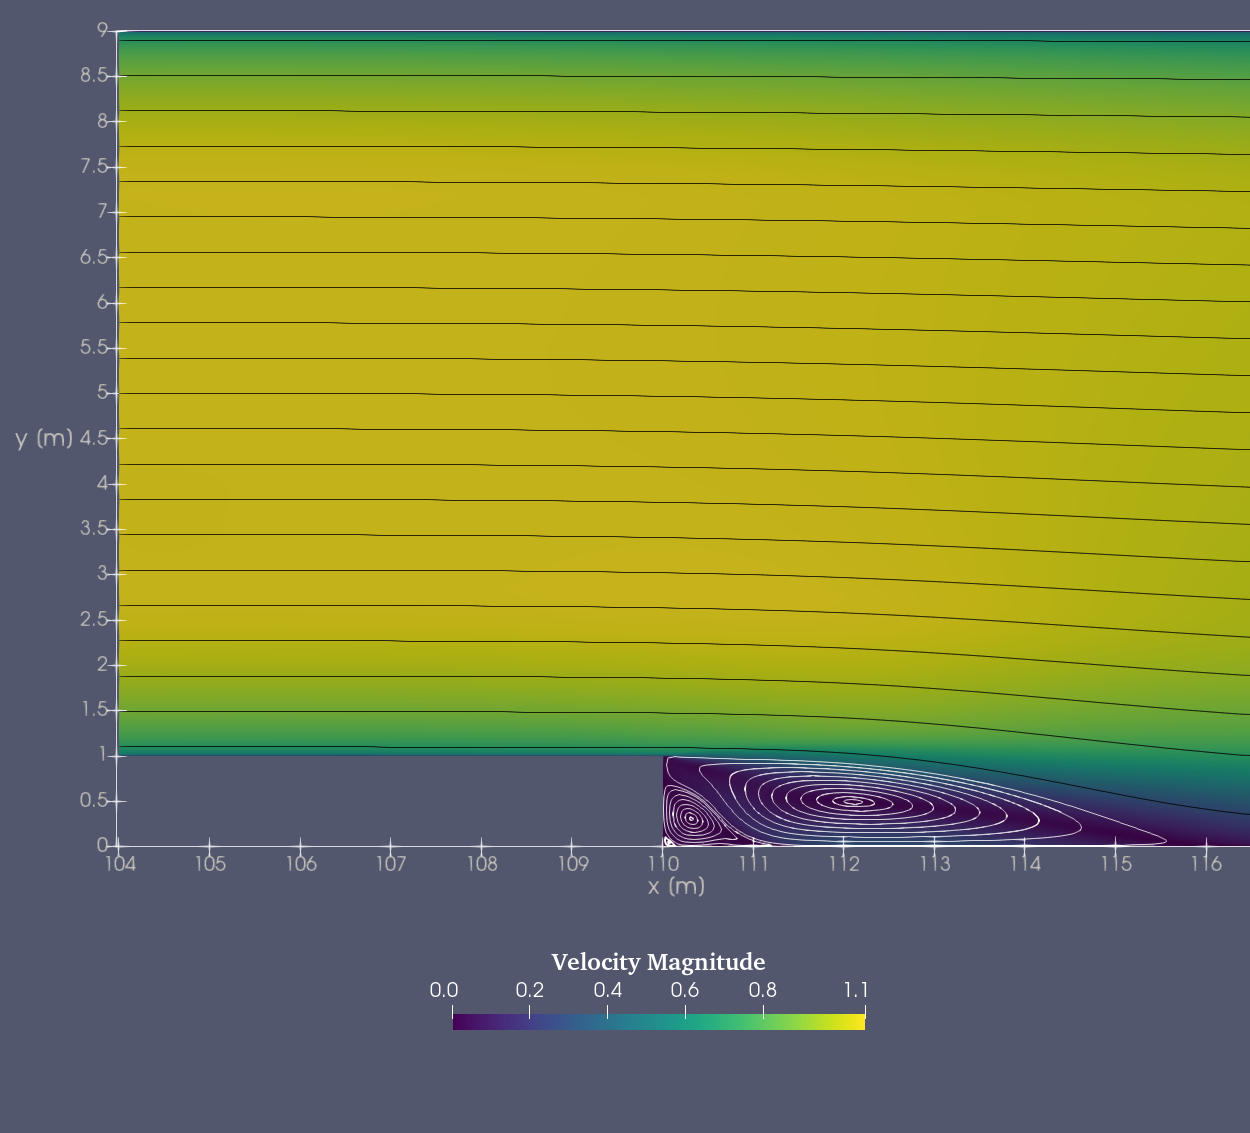
\includegraphics[width=\columnwidth]{bfs}
  \caption{}
  \label{fig:}
\end{figure}

% !media bfs_upstream_vel.png
%        id=bfs-upstream-vel
%        caption=Normalized velocity distribution at $x/H$ equal -4 (upstream of step).
%        style=width:33%;padding:10px;float:left;
% 
% !media bfs_downstream_vel.png
%        id=bfs-downstream-vel
%        caption=Normalized velocity distribution at various $x/H$ locations (downstream of step).
%        style=width:33%;padding:10px;float:left;
% 
% !media bfs_cf.png
%        id=bfs-cf
%        caption=Skin friction coefficient along the bottom wall.
%        style=width:33%;padding:10px;float:left;
% 
% !media bfs_cp.png
%        id=bfs-cp
%        caption=Skin pressure coefficient along the bottom wall.
%        style=width:33%;padding:10px;margin-left:17%;float:left;
% 
% !media bfs_stress.png
%        id=bfs-stress
%        caption=Normalized turbulent shear stress distribution at various $x/H$ locations
%        (downstream of step).
%        style=width:33%;padding:10px;margin-right:17%;float:left;
% 
% !media bfs.png
%        id=bfs
%        caption=Close-up of the velocity magnitude and streamlines around the backward-facing step
%        style=width:80%;float:left;margin-left:10%;margin-right:10%;
